\documentclass{beamer}
\usetheme{UPJR}
\usepackage[orientation=portrait,size=a0,scale=1.4]{beamerposter}
\usepackage{fp}
\usepackage{bg}

\usepackage{xkeyval}
\usepackage{type1cm}
\usepackage{paralist}
\usepackage[spanish]{babel}
%\usepackage[latin1]{inputenc}
\usepackage[utf8]{inputenc}
\usepackage[T1]{fontenc}
\usepackage{lmodern}
\usepackage{textcomp}
\usepackage{amsmath}
\usepackage{graphicx}
\usepackage{textpos}
\usepackage{ragged2e}
\usepackage{verbatim}
 \usepackage{wrapfig} %Inclusión de gráficos al lado de texto
 \usepackage[rflt]{floatflt} %Para meter figuras flotantes entre el texto
%\decimalpoint

\title{Tech-tuin}
\author{Aide Pizano Escalante, Cristian Iván Muñiz Mendoza, Elías Abraham Ramírez Rivera, José Martin Nieto León, Víctor Alfonso Humareda Barbosa}
\institute{Ingeniería en Telemática}
\footer{}
\date{}

\begin{document}
\begin{frame}[fragile]{} 
\begin{columns}[t]
  \begin{column}{0.46\textwidth}
    \begin{block}{Introducción}\justifying
      Década a década la cantidad de agua potable en México se ve disminuida debido al desperdicio inconsciente de la misma. Tan solo en Guanajuato, un habitante promedio consume alrededor de 87 litros al día. siendo aproximadamente 50 \% no reutilizable. Entre las actividades donde se presenta un mayor consumo de agua se encuentra el riego de jardines domésticos por lo que, la implementación de un sistema de riego automatizado ayuda a dar un uso más racional del agua, logrando en el proceso una mejora en la condición del jardín.\\
      \textbf{Palabras Clave:} \textit{ jardín, sistema de riego, automatización}
     \end{block}
  \end{column}
  \begin{column}{0.46\textwidth}
    \begin{block}{Objetivo}\justifying
        Desarrollar e implementar un sistema de riego automático que reduzca el consumo
agua al momento de regar jardines domésticos, utilizando un circuito electrónico que sea
capaz de tomar decisiones basado en las condiciones ambientales del jardín. \\

    \end{block}
  \end{column}
\end{columns}

\vspace*{\stretch{1}}

\justifying
\begin{columns}[t]
 \begin{column}{0.96\textwidth}
     \begin{block}{Marco Teórico}
           \vspace{0pt}
 Sistema de riego es el conjunto de estructuras que permite determinar qué área debe ser regada a partir de ciertas condiciones, aplicándole el agua necesaria a las plantas. Este consta de varios componentes. El conjunto dependerá de si se trata de riego superficial, por aspersión, o por goteo. Donde existen diferentes sistemas de riego por ejemplo:
\begin{itemize}
\item  Riego por aspersión.
\item  Riego por goteo automático
\item  Riego de superficie.
\end{itemize}
Estos riegos son manipulados manualmente por personas sin embargo, el instalar un sistema de riego tiene ventajas tales como:

\begin{itemize}

\item Se logran altos grados de automatización, basados en el ahorro de mano de obra,
agua y energía.
\item Los equipos son adaptables a cualquier tipo de terreno.

\item Estos sistemas son adaptables a la rotación de plantas y a riesgos estratégicos.
\item Permite el crecimiento vertical de las plantas.


\end{itemize}
    \end{block}
  \end{column}
\end{columns}

\vspace*{\stretch{1}}

\justifying
\begin{columns}[t]
	
	
	  \begin{column}{0.46\textwidth}
	  	\begin{block}{Estudio de mercado}
	  		\begin{minipage}[t]{1\linewidth}
	  			\vspace{0pt} 
Potencial de mercado:

\begin{itemize}
\item 20,144 casas habitadas con jardín
\item Tamaño de la muestra: 96
\item Margen de error: 10\%
\item Fiabilidad: 95\% \\
Estos fueron los datos que se obtuvieron con la encuesta aplicada a un grupo de personas, donde también se interpretaron otros datos como los siguientes.
\item Entre los datos se obtuvieron en la aplicación de la encuesta, se observó que un 94\%, le interesaría tener un sistema de riego automático en su hogar.
\end{itemize}
\begin{figure}[H]
	\centering
	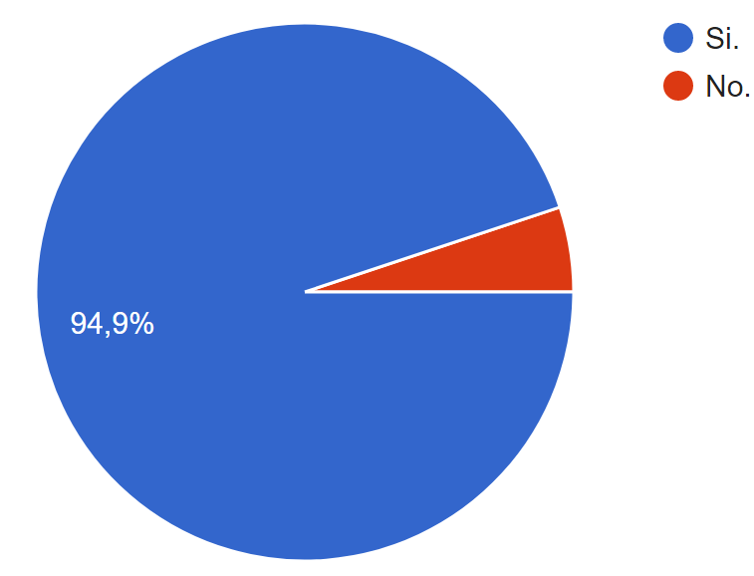
\includegraphics[scale=0.7]{../graphics/Imagen1.png}
\end{figure}

\end{minipage} 
	  	\end{block}
	  \end{column}
	
	 \begin{column}{0.46\linewidth}
	 	\begin{block}{Descripción del proyecto}
	 	
	 	
Es un sistema de riego automático que tomará decisiones para regar, con base a los datos que obtenga de los sensores, comparándolos a su vez con la información que se encuentre en la base de datos para así tomar la decisión de regar o no regar. La información de los sensores se guarda en la base de datos para tener registro de los mismos y mostrársela al usuario.
\begin{figure}[H]
	\centering
	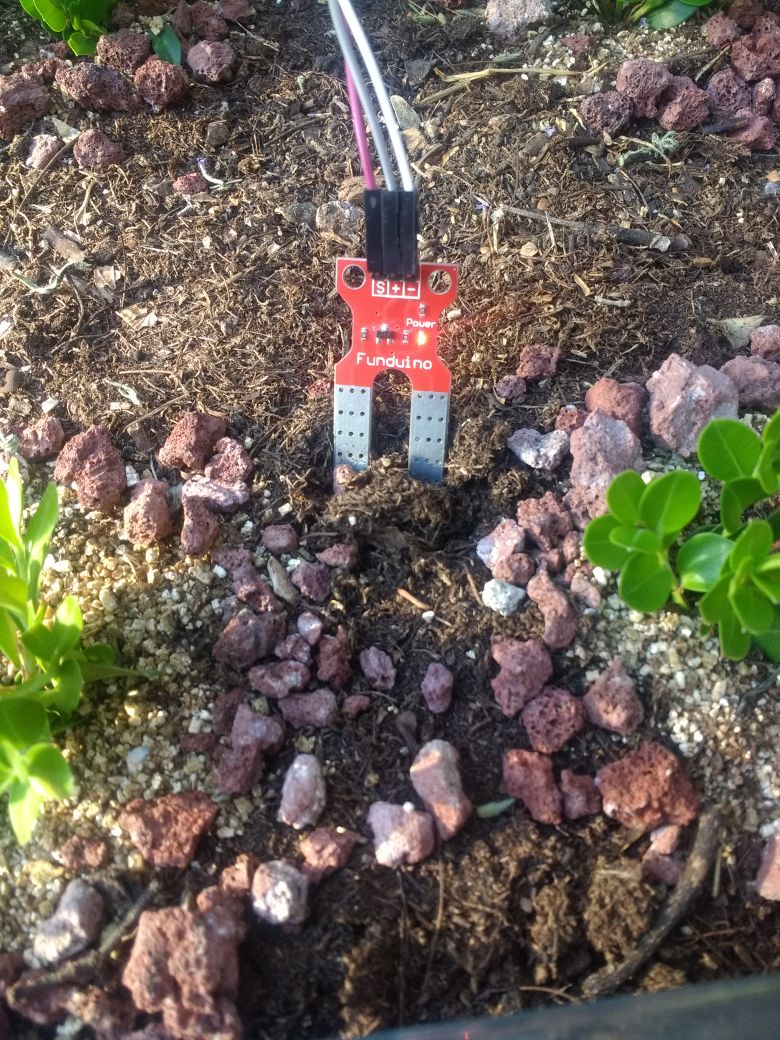
\includegraphics[scale=0.5]{../graphics/s2}
\end{figure}
	 	 
	 	\end{block}
	 \end{column}
	\end{columns}
 
 	\vspace*{\stretch{1}}
 	\justifying
 	\begin{columns}[t]
 
  
  \begin{column}{0.46\linewidth}
  	\begin{block}{Trabajo a futuro}
  		\begin{minipage}[t]{1\textwidth}
  			\vspace{0pt}
 Se pretende incluir más sensores al prototipo para el monitoreo de las plantas. Reemplazar el arduino por pics para reducir el costo del proyecto y por último, conectar el sistema a internet para que el usuario analice la información.
  		\end{minipage} 
  	\end{block}
  \end{column}

	     \begin{column}{0.46\linewidth}
	     	\begin{block}{Conclusiones y trabajo futuro}\justifying
	     		\begin{minipage}[t]{0.96\textwidth}
	     			\textbf{Conclusiones}: 
	     			Durante la investigación, se obtuvo que, contar con un sistema de riego automático para jardines es viable principalmente en México ya que es uno de los países donde más se consume agua,el sistema de riego automático ayuda a dar un uso más racional del agua y a mejorar la condición del jardín.
	     			\\
	     			
	     		\end{minipage}
	     		
	     	\end{block}   
	     \end{column}
\end{columns}

\vspace*{\stretch{1}}
\justifying
\begin{columns}[t]
 \begin{column}{0.96\linewidth}
      \begin{block}{Referencias}
	\begin{minipage}[t]{0.71\textwidth}
        \begin{small}
        \begin{thebibliography}{widestlabel}
        	\bibitem{Jardinería} Gil-Albert V. F,(2006),Manual técnico de jardinería I. Establecimiento de jardines,
parques y espacios verdes, Madrid España, Mundi-prensa
        	\bibitem{arduino} Sistema de Riego Inteligente para Optimizar el Consumo de
Agua. Panama: Universidad Tecnológica de Panama.

        	\bibitem{Agricultura} Francisco Miguel Aguila Marın. (2008). Agricultura Técnica en México. Mexico: Universidad Hohenheim.
        	
        	
        	\bibitem{riego} Martín Tarjuelo. (2010). El riego y su tecnología. México: Mundi-Prensa
        	
        \end{thebibliography}
        \end{small}
        \end{minipage}
        \hfill
           \begin{minipage}[t]{0.25\textwidth}
           	\vspace{0pt}
           	\begin{center}
           		\begin{figure}
           			
\includegraphics[scale=0.2]{../graphics/ite.png} 
           		\end{figure}
           	\end{center}
           \end{minipage}
      \end{block}
   \end{column}
\end{columns}

\end{frame}
\end{document}
